% !TEX root = ../Abschlussbericht_Schimmeliger_Keller.tex
%%
%%  Hochschule für Technik und Wirtschaft Berlin --  Projektabschlussbericht
%%
%% Kapitel 2 - Vorbereitung und Konzeptentwicklung
%%
%%

\chapter{Projektplanung} \label{Projektplanung}
\section{Pflichtenheft} \label{Pflichtenheft}

Auch wenn wir in erster Linie ein Produkt aus freien Inhalten entwickeln wollen, müssen wir an einigen Stellen den Kompromiss zwischen freiem Inhalt und Entwicklungsaufwand eingehen, da wir in der zeitlichen Ressource begrenzt sind.
Im Zuge der Projektplanung haben wir eine Umfrage durchgeführt, woraus sich unser Pflichtenheft abgeleitet hat.

\begin{itemize} 
	\item \textbf{Anschaffungskosten:} Unser Persona möchte maximal 40 Euro in dieses Projekt investieren, um einen funktionsfähigen Funksensor zu erhalten. 
	
	\item \textbf{Laufende Kosten:} Um die laufenden Kostn gering zu halten, soll der Funksensor möglichst stromsparend und wartungsarm sein. Die Hardware sollte ihren Strom über einen Akku bzw. eine Batterie beziehen.
	
	\item \textbf{Einsatzgebiet:} Da der Sensor am Mikrocontroller im Bereich von -40°C\dots80°C arbeitet und auch in Gebieten mit einer relativen Feuchtigkeit von bis zu 100\% zum Einsatz kommen soll, muss das fertige Endprodukt mindestens diesen Anforderungen entsprechen. Die Entwicklung eines Gehäuses erfolgt aber erst nach Erreichen der Serienreife.
	
	\item \textbf{Datenschutz:} Der Endnutzer möchte selbst bestimmen, ob und mit wem er seine gesammelten Daten teilt. Des weiteren möchte er selbst bestimmen, ab welchem Zeitpunkt/Schwellwert er über den aktuellen Datenstand informiert wird.

\end{itemize}


\subsection{Vorgangsmodell} \label{Vorgangsmodell}
Scrum ist ein Vorgehensmodell im Projektmanagement, welches seinen Ursprung in der Softwareentwicklung hat.
Der Ansatz von Scrum ist das systematische Sammeln von Erfahrungen (empirisch), das kontinuierliche weiterentwickeln bestehender Module (inkrementell), sowie dem mehrfachen Wiederholen gleicher oder ähnlicher Prozesse (iterativ) und basiert auf der Erkenntnis, dass viele Entwicklungsprojekte zu komplex sind, um sie in einem vollumfänglichen Plan fassen zu können, was wiederum den Grund hat, dass wesentliche Teile der Ursprungsanforderung bzw. deren Lösungsansätze zu beginn unklar sind.

Ein weiteres Merkmal von Scrum ist, dass neben dem Produkt auch die Planung kontinuierlich verändert bzw. weiterentwickelt, wobei der langfristige Plan, auch Product Backlog genannt, iterativ verfeinert und verbessert wird.

Resultierende Arbeitspakete werden zyklisch in sogenannten Sprints detailliert formuliert und in einem Detailplan, auch Sprint Backlog genannt, zur Bearbeitung abgelegt, sodass diese, fokussiert auf die aktuelle Problemstellung, abgearbeitet werden können.

Ziel ist dabei eine schnelle und kostngünstige Entwicklung hochwertiger Produkte, wobei die jeweiligen Anforderungen aus der Anwendersicht formutliert werden.

\begin{figure}[h]
 \centering
 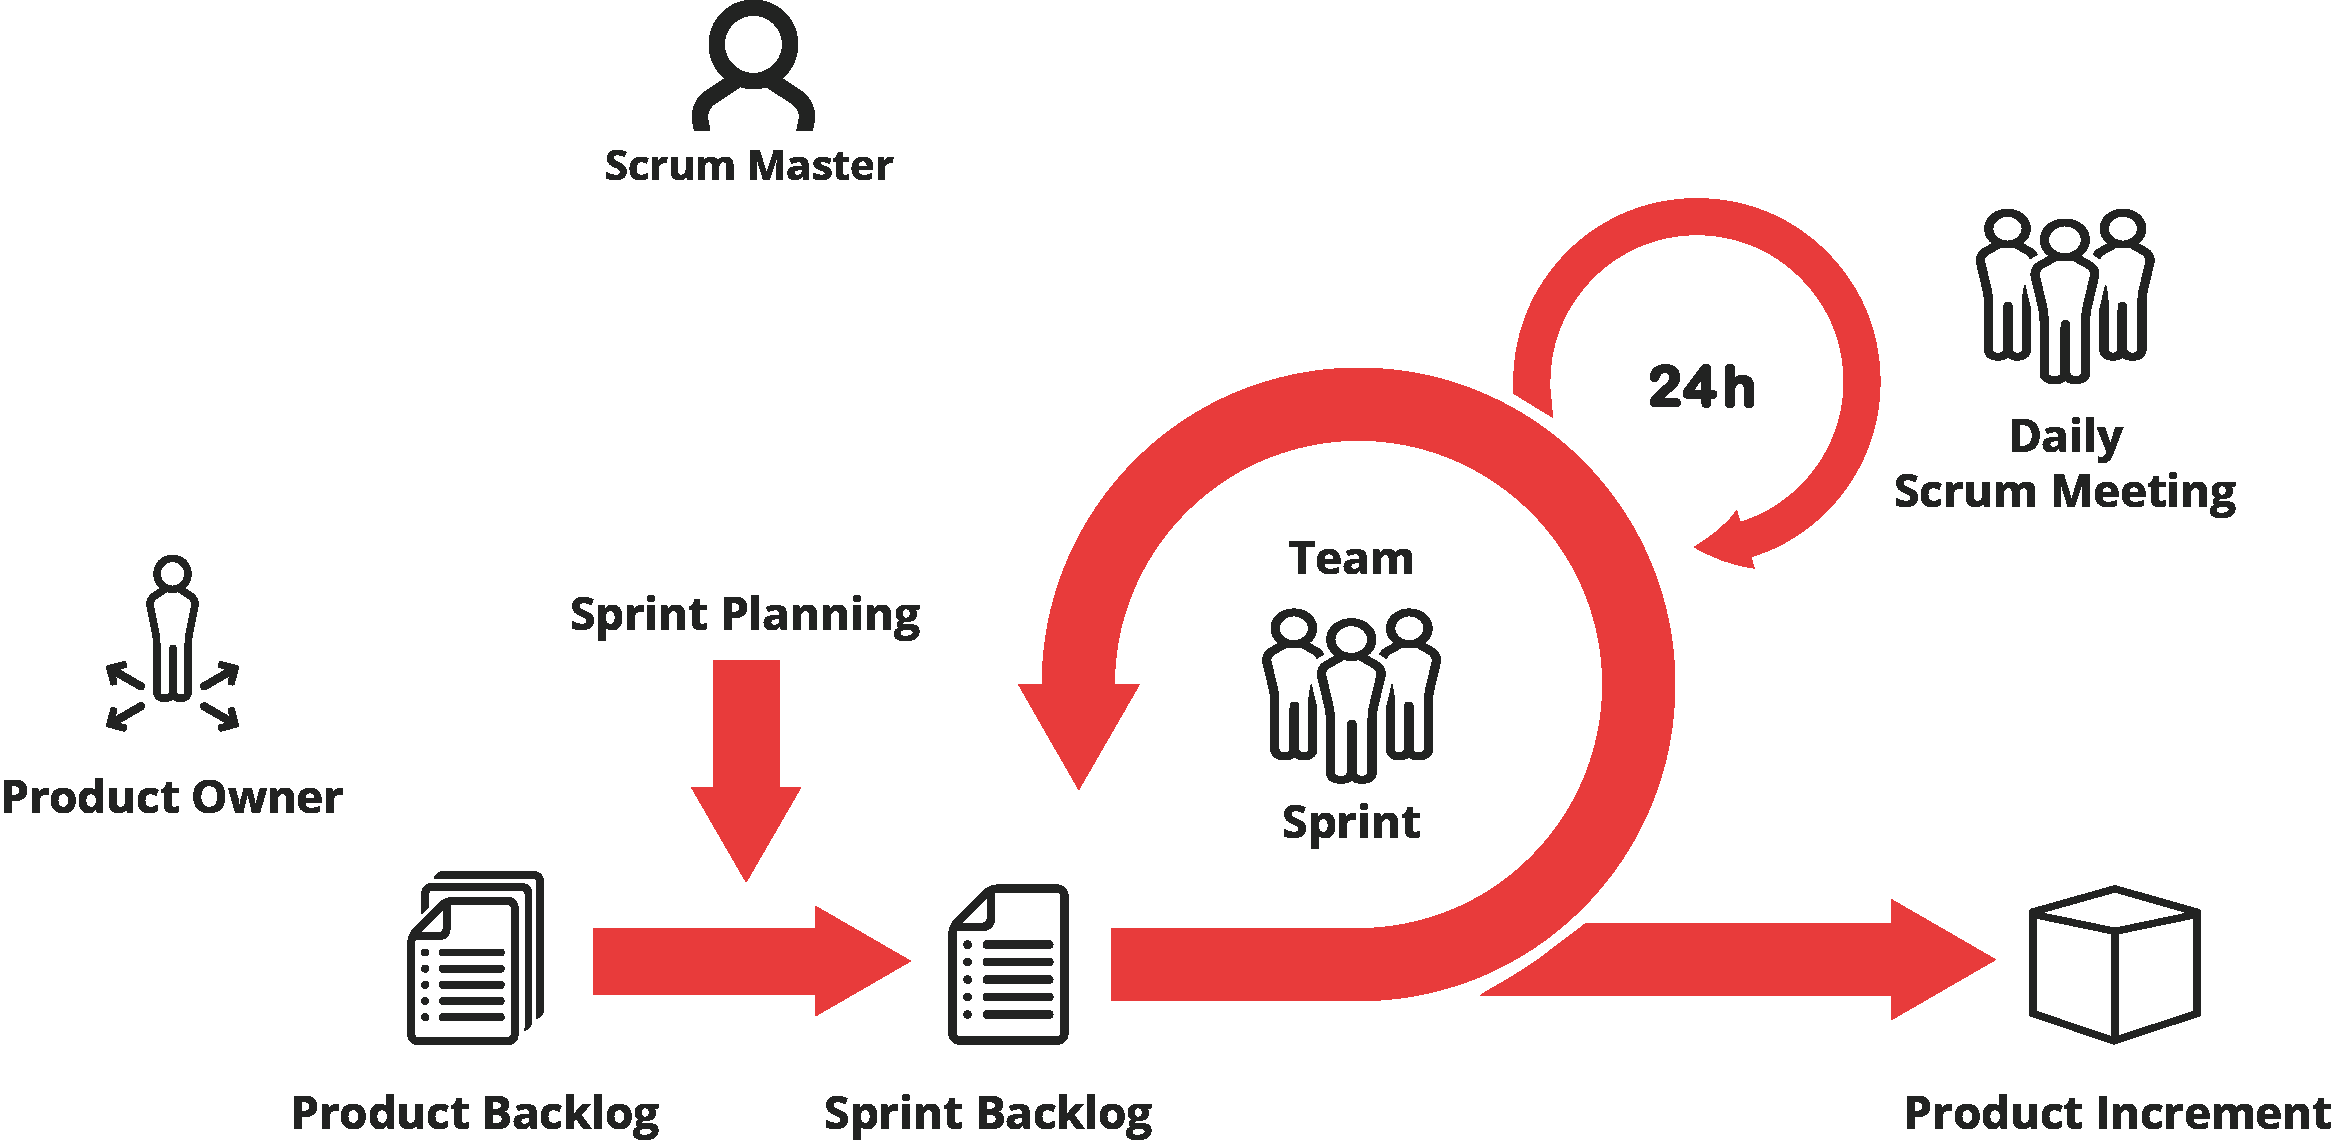
\includegraphics[width=0.8\textwidth]{pictures/scrum}
 \caption[Agiles arbeiten mit Scrum]{Agiles arbeiten mit Scrum } %%\cite{scrum2018}
 \label{fig:scrum}
\end{figure}

Die Verantwortlichkeiten liegt beim sogenannten Scrum-Team, welches sich aus folgenden Rollen ergibt:
\begin{adjustwidth}{-1in}{-1in}% adjust the L and R margins by -1 inch
	\begin{center}
		\begin{tabular}{ ccc }
			\toprule
			{Rolle} & {Besetzung in unserem Projekt} & {Anmerkung}\\
			
			\midrule
			{Product Owner} & {HTW Berlin} & {Vertreten durch Prod. Dr. Thomas Scheffler}\\
			{Scrum Master} & {-} & {-}\\
			{Projektmanager} & {Sidney Göhler} & {-}\\
			{Scrum Team} & {Sidney Göhler, Ilja Buschujew} & {-}\\
			\bottomrule
		\end{tabular}
		\captionof{table}{Verantwortlichen im Scrum-Team} \label{tab:scrumverantwortung} 
\end{center}
\end{adjustwidth}


\newpage

\subsection{Projektstruktur} \label{Projektstruktur}

Aus den uns gesetzten Pflichten, haben sich für uns die folgende Projektstruktur grob herauskristalisiert, welche im laufenden Prozess immer weiter in Arbeitspakete verfeinert wurde.


\begin{center}
	\begin{figure}[h]
		 \noindent\makebox[\textwidth]{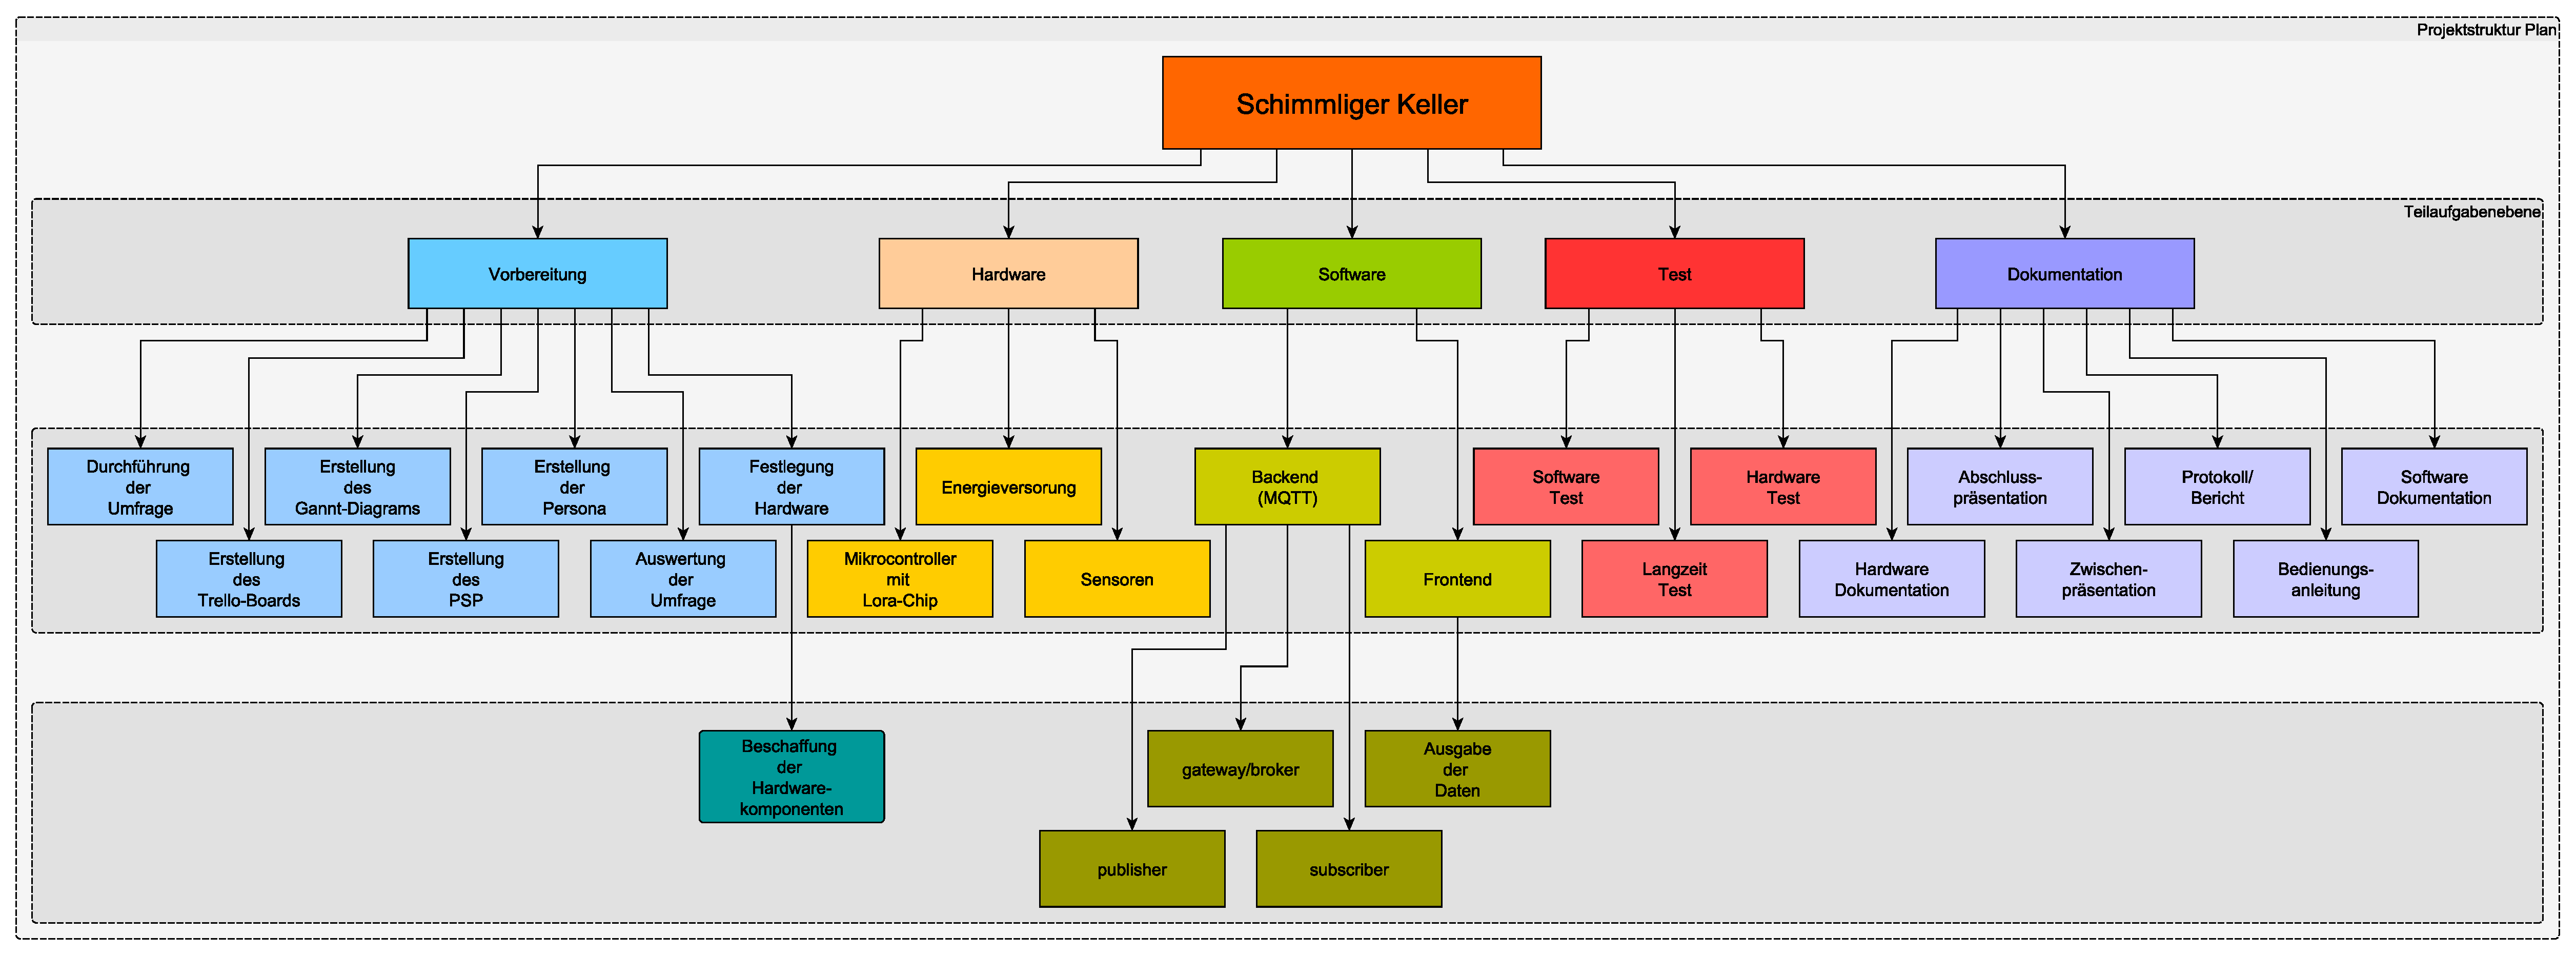
\includegraphics[width=1.2\textwidth]{pictures/PSP}}
		 \caption[Projektstrukturplan]{Projektstrukturplan} %%\cite{scrum2018}

	\end{figure}
\end{center}

Mithilfe des Projektstrukturplanes ließen

\subsection{Zeitplanung} \label{Zeitplanung}

\begin{center}
	\begin{figure}[h]
	 
	 \noindent\makebox[\textwidth]{
\includegraphics[width=1.3\textwidth]{pictures/zeitplanung}}
	 \caption[Übersicht unserer Zeitplanung]{Übersicht unserer Zeitplanung} %%\cite{scrum2018}
	 \label{fig:zeitplanung}
	\end{figure}
\end{center}

Illustriert wird unsere grobe Zeitplanung zu Beginn des Projektes. Wir wollten aufgrund unserer agilen Arbeitsweise nur grobe Zeiträume definieren. Wie sich schlussendlich herausgestellt hat, haben manche Teilaspekte länger, andere wiederum kürzer gerdauert.

\newpage
Nachfolgend wird eine tabellarische Übersicht unserer Zeitplanung aufgeführt, wobei wir die Daten aus unserem Trello-Board entnehmen:
\begin{adjustwidth}{-1in}{-1in}% adjust the L and R margins by -1 inch
	\begin{center}
		\begin{tabular}{ ccccc }
			\toprule
			{Vorgangsname} & {Anfang} & {Ende} & {Bearbeiter} & {Arbeitszeit}\\
			
			\midrule
			\multicolumn{5}{c}{\textbf{Vorbereitung}} \\
			{Sichtung der Quellenlage} & {01.10.2021} & {20.02.2022} & S + I & 20h\\
			{Erstellung Trelloboard} & {01.10.2021} & {01.10.2021} & S & 30m\\
			{Erstellung eines Git repositories} & {01.10.2021} & {01.10.2021} & S & 30m\\
			{Erstellung des PSP} & {01.10.2021} & {20.02.2022} & I & 2h\\
			{Erstellung Zeitplan} & {01.10.2021} & {20.02.2022} & S & 2h\\
			{Erstellung/Durchführung der Umfrage} & {01.10.2021} & {02.12.2021} & S + I & 20h\\
			{Festlegung/Beschaffung der Hardware} & {01.10.2021} & {20.02.2022} & S + I & 20h\\
			{Auswahl/Einrichtung Software IDE} & {01.10.2021} & {20.02.2022} & S + I & 20h\\
			{Auswertung der Umfrage} & {01.10.2021} & {20.02.2022} & S + I & 20h\\
			{Erstellung des Persona} & {01.10.2021} & {20.02.2022} & S + I & 20h\\

			\midrule
			\multicolumn{5}{c}{\textbf{Hardware}} \\
			{Inbetriebnahme der Hardware} & {01.10.2021} & {20.02.2022} & S + I & 20h\\

			\midrule
			\multicolumn{5}{c}{\textbf{Software}} \\
			{µC Management} & {01.10.2021} & {20.02.2022} & S + I & 20h\\
			{Integration der Sensoren} & {01.10.2021} & {20.02.2022} & S + I & 20h\\
			{Einrichtung einer P2P LoRa-Kommunikation} & {01.10.2021} & {20.02.2022} & S + I & 20h\\
			{Entwicklung eines MQTT Publishers} & {01.10.2021} & {20.02.2022} & S + I & 20h\\
			{Entwicklung eines MQTT Subscribers} & {01.10.2021} & {20.02.2022} & S + I & 20h\\
			{Einrichtung einer grafischen Schnittstelle} & {01.10.2021} & {20.02.2022} & S + I & 20h\\
			{Softwaretests} & {01.10.2021} & {20.02.2022} & S + I & 20h\\

			\midrule
			\multicolumn{5}{c}{\textbf{Nachbereitung}} \\
			{Vorbereitung der Zwischenpräsentation} & {01.10.2021} & {20.02.2022} & S + I & 20h\\
			{Vorbereitung der Abschlusspräsentation} & {01.10.2021} & {20.02.2022} & S + I & 20h\\
			{Dokumentation} & {01.10.2021} & {20.02.2022} & S + I & 20h\\
			{Langzeittests} & {01.10.2021} & {20.02.2022} & S + I & 20h\\

			\bottomrule
		\end{tabular}
		\captionof{table}{Übersicht der Arbeitspakete und Arbeitszeiten} \label{tab:worklog} 
	\end{center}

\end{adjustwidth}

\newpage

\subsection{Kostenaufstellung} \label{Kostenaufstellung}

Auch wenn wir unser Projekt in erster Linie als Freie Software bereitstellen wollen
Aus unseren Anforderungen geht hervor, dass die meisten potentiellen Nutzer möglichst wenig für unser Produkt bezahlen möchten. Wie bei 

\begin{adjustwidth}{-1in}{-1in}% adjust the L and R margins by -1 inch
	\begin{center}
	
	        \begin{tabular}{ccc|ccc}
			\toprule
			\multicolumn{3}{c}{\textbf{PyCom}} & \multicolumn{3}{c}{\textbf{DIY}}\\
	
			Name & Anzahl & Kosten & Name & Anzahl & Kosten\\

			\midrule
			LoPy4 & 1 & 38,45 & ESP32 DevKit & 1 & 9,99\\
			Pytrack  & 1 & 40,65 & Breadboard & 1 & 5,99\\
			Antennen-Kit  & 1 & 9,00 & LoRa Transceiver + Antenne & 1 & 11,98\\
			3 X 1.5V AAA Batterie-Halterung & 1 & 9,00 & 3 X 1.5V AAA Batterie-Halterung & 1 & 9,00 \\
			DHT22 Sensor & 1 & 9,99 & DHT22 Sensor & 1 & 9,99\\
			 &  &  & Passive Bauelemente &  & 2,00\\

			\midrule
			\textbf{Gesamtkosten} & & 107,09 & \textbf{Gesamtkosten} & & 48,95\\

			\bottomrule
	
	        \end{tabular}
		\label{}
		\captionof{table}{Kostenaufstellung für das Projekt} \label{tab:kostenaustellung} 
	\end{center}
\end{adjustwidth}

Anzumerken ist hier, dass die Entwicklung des Produktes mithilfe der PyCom Plattfrom zwar deutlich kostenintensiver ist, aber besonders für einen Prototypen doch recht komfortabel, da jeder einzelne Baustein dafür gemacht ist, miteinander zu funktionieren.\\
Tendenziell ließe sich aber mit einem "Selbstbau" der Preis um knapp die hälfte reduzieren.\\
Neben der PyCom Plattform existieren noch andere Entwicklungsplattformen, wie z.B. das \textit{TOOGOO WiFi ESP-32 Entwicklungs Board}, welches den LoRa Transreceiver implementiert und teilweise auch schon eine Halterung für Batterien anbietet. 


\section{Systemkonzept und theoretische Realisierung} \label{Systemkonzept und theoretische Realisierung}

\subsection{Systemkonzept} \label{Systemkonzept}



